Boom hacka lacka

\subsection{Shadows}
Shadows are one those things that can make a scene really come to life. It will help the viewer to understand the structure of the terrain and location of objects much better than with only shading. There are many techniques in which shadows can be achieved with different pros and cons. We have chosen to use \textit{Shadow Mapping} \cite{ShadowMapping} which by now is a fairly old technique, 1978, but still used in many modern computer games. Shadow mapping offers real-time shadows for arbitrary scenes in a theoretically straight forward way. 

The quality of these shadows can be increased arbitrarily, but the computational complexity grows linearly with the size of the rendered screen \cite{ShadowMapping}. Therefor one has to limit this size and go for a number of improvement techniques to make shadows shine. 

More specifically our implementation utilizes \textit{Light Space Perspective Shadow Mapping} \cite{LSPShadowMapping} which can be summarized in the following steps:

\begin{itemize}
\item Place the camera in the light source and adjust the camera frustum to cover the part of the scene that will be visible in the final render.
\item Render the scene with as simple shaders as possible and store the depth buffer. This is the shadow map.
\item Place the camera in its final-render location.
\item For each vertex:
\begin{itemize}
\item Transform into light-space coordinates.
\item Compare the distance from the light source with the corresponding value in the shadow map.
\item If the vertex is further away than the shadow map suggests, it will be shadowed. 
\end{itemize}
\end{itemize}

Once these steps got into place one could naively think that the shadows are done once and for all, but thats not the case. The result out-of-the-box looks something like figure \ref{fig:SMAcne}. The terrain is full of errors and the shadows have a pretty bad resolution. The erroneous self-shadowing on the terrain is called \textit{Shadow Acne} \cite{ImprovedShadowMapping} and is caused by precision errors in the depth test. The value in the depth map and the real depth are too close so the depth test randomly fails. This can be fixed by adding an offset to the depth value which will remove the shadow if the two depth values are too close. The improved result can be seen in figure \ref{fig:SMAcneFix}.

\begin{figure}[H]
\begin{subfigure}{.5\textwidth}
  \centering
  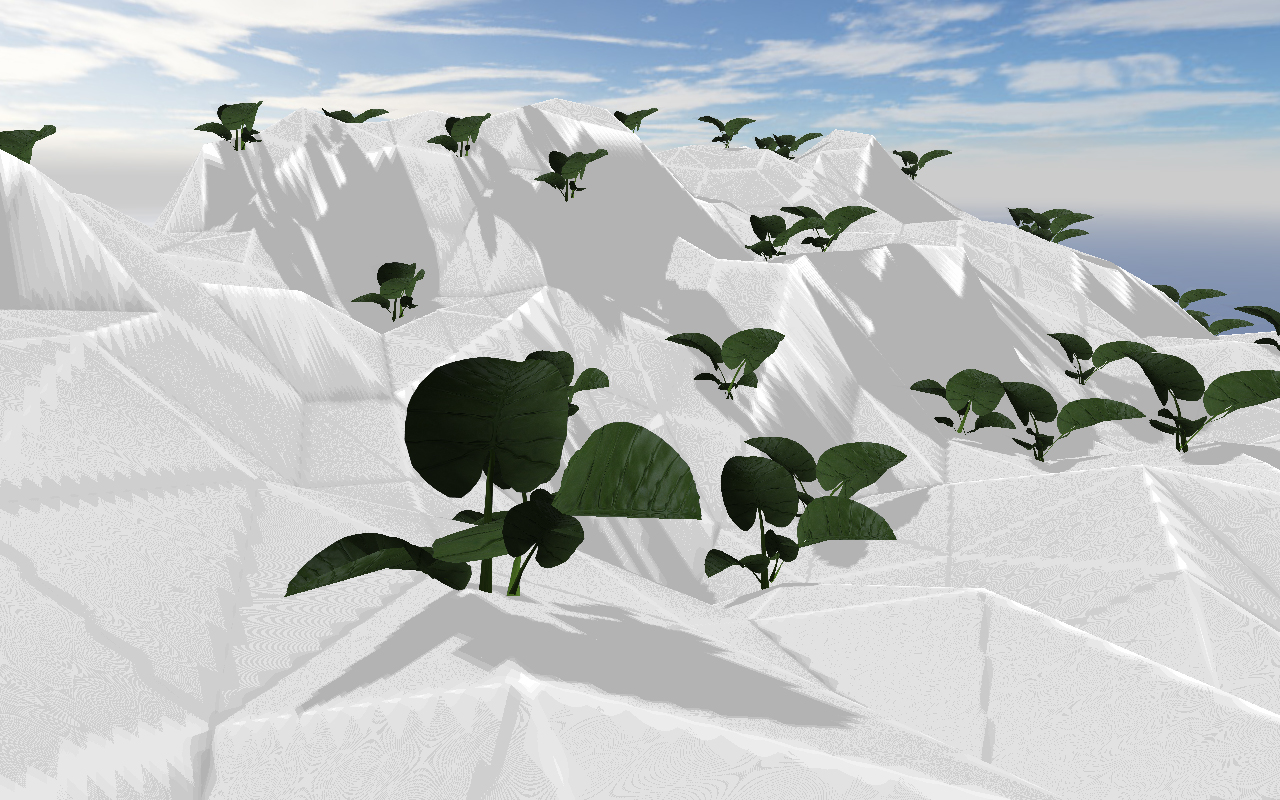
\includegraphics[width=0.9\linewidth]{images/SMAcne.jpg}
  \caption{Surface suffering from severe acne}
  \label{fig:SMAcne}
\end{subfigure}%
\begin{subfigure}{.5\textwidth}
  \centering
  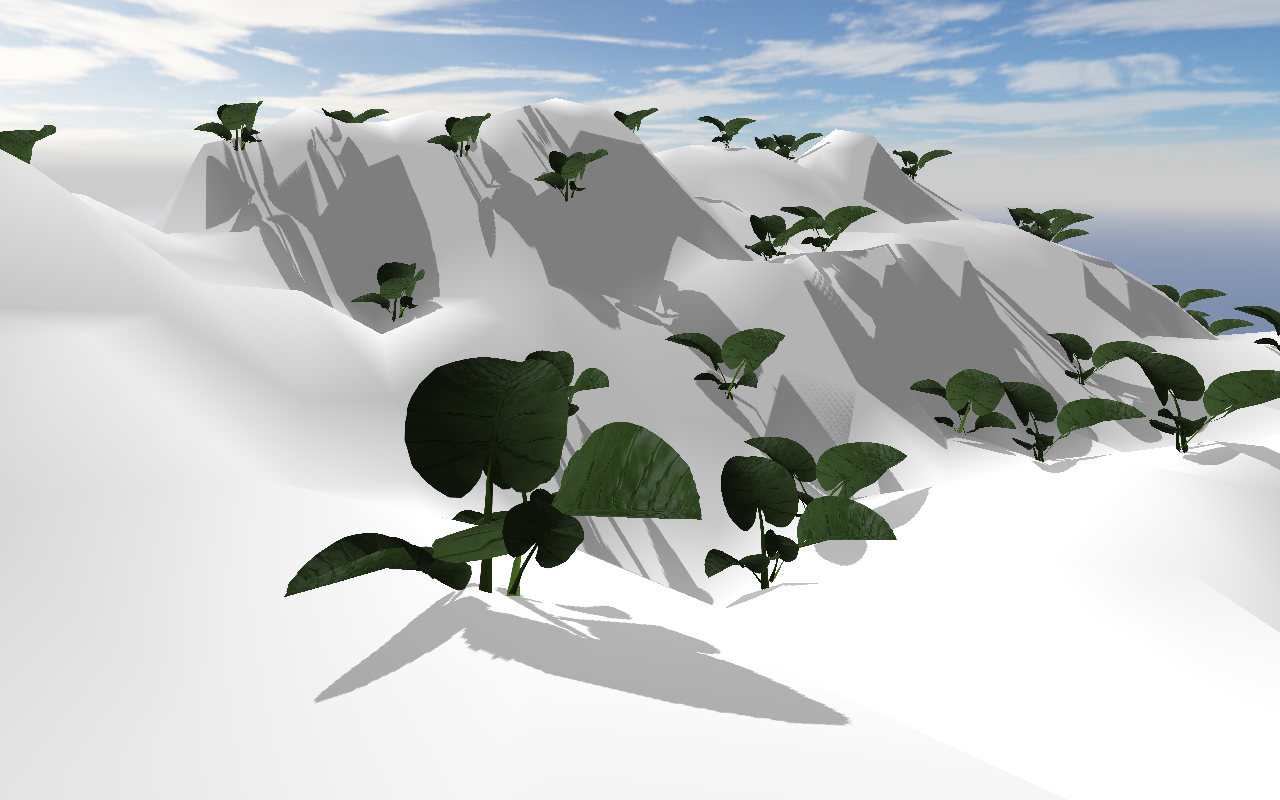
\includegraphics[width=0.9\linewidth]{images/SMAcneFix.jpg}
  \caption{Surface healed by addition of small offset}
  \label{fig:SMAcneFix}
\end{subfigure}
\caption[Shadow mapping, acne comparison]{\textit{Comparison of shadow mapping with and without acne}}
\label{fig:AcneComparison}
\end{figure}

Care has to be taken when adding this depth offset. If the offset is to large the shadow may be disconnected from its object and cause so called \textit{Peter Paning} \cite{ImprovedShadowMapping}. A trade-off has to be made between Shadow Acne and Peter Paning. Thanks to good resolution in our depth buffers we did not need any big offset to remedy our acne problem and did therefore not suffer from any noticeable Peter Paning. 

The shadows now look correctly but have a very low resolution when you get close up. The edge is sharp and one can easily distinguish pixels in a not so pleasant may. Increasing the resolution of the shadow map depth buffer will reduce the pixel size of the shadows in the final render but this will decrease the frame rate. We settled on 2048 x 2048 pixels in our buffer, figure \ref{fig:PCFLvl1}. Now my first thought was to low pass filter the shadow map, and this is sort of used in the improvement technique called \textit{Percentage Closer Filtering} (PCF) \cite{ShadowMapAntialiasing87}\cite{ShadowMapAntialiasing03}. By randomly sampling the surroundings of the target shadow map pixel and weighting them, in our case with a Gaussian kernel in accordance with \cite{CascadeShadowMapping}, one get a smoother shadow edge. The result is definitely a good looking improvement, figure \ref{fig:PCFLvl5}. 

\begin{figure}[H]
\begin{subfigure}{.5\textwidth}
  \centering
  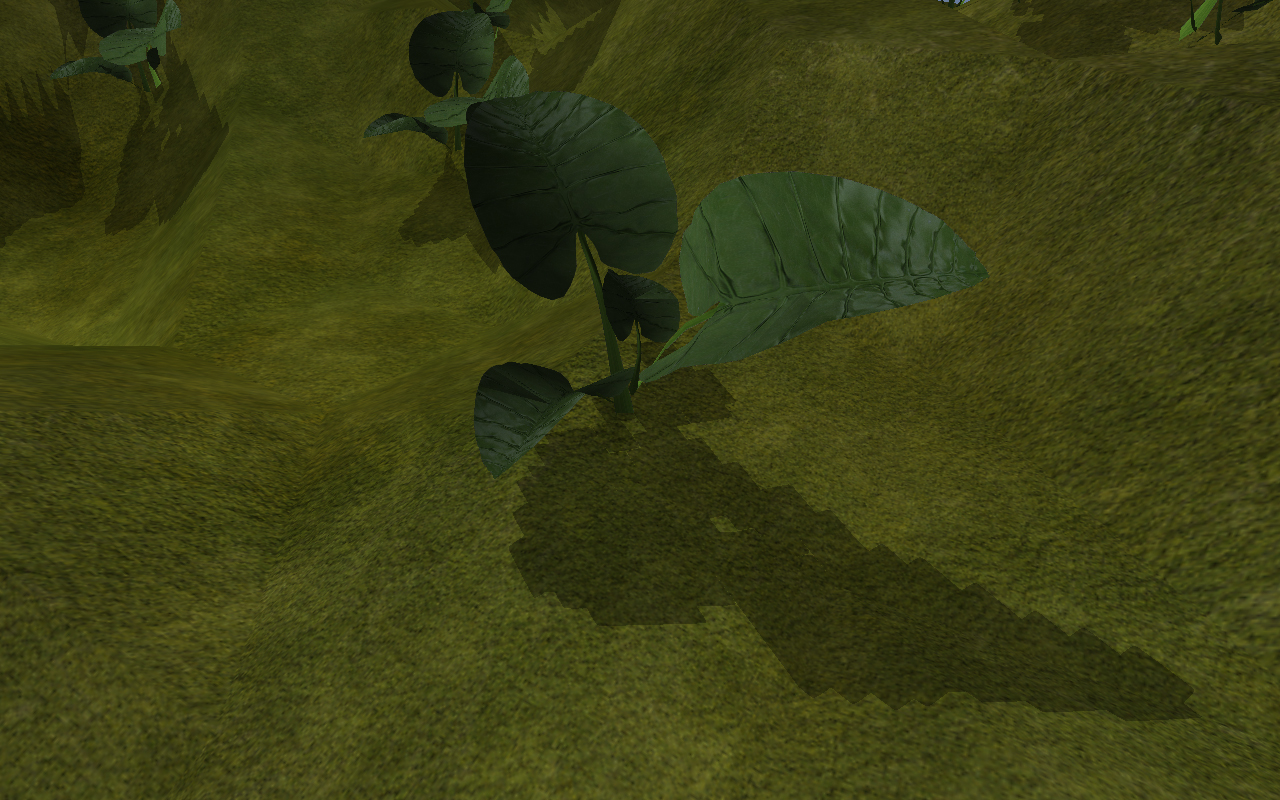
\includegraphics[width=0.9\linewidth]{images/PCFLvl1.jpg}
  \caption{Out-of-the-box shadows}
  \label{fig:PCFLvl1}
\end{subfigure}%
\begin{subfigure}{.5\textwidth}
  \centering
  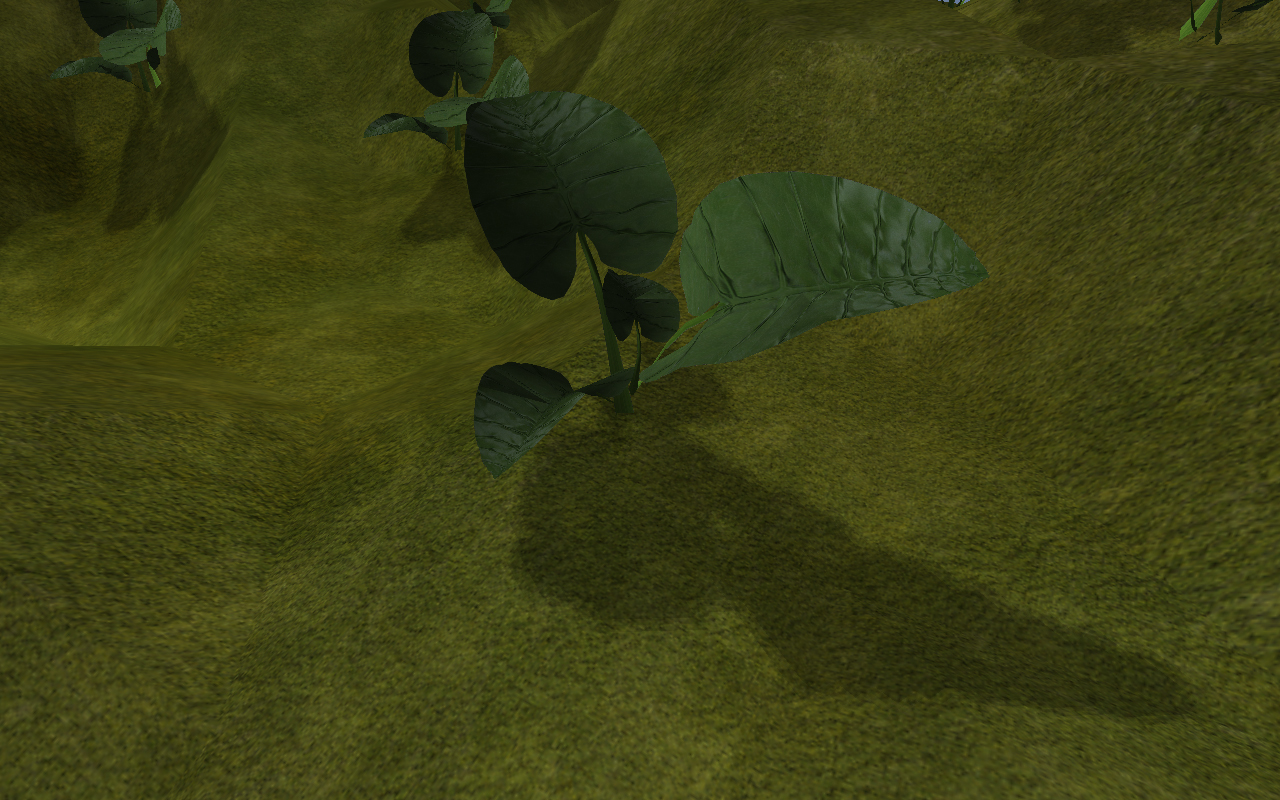
\includegraphics[width=0.9\linewidth]{images/PCFLvl5.jpg}
  \caption{Percentage closer filtered shadows}
  \label{fig:PCFLvl5}
\end{subfigure}
\caption[Noise comparison]{\textit{Comparison of shadow mapping with and without percentage-closer filtering}}
\label{fig:PCFComparison}
\end{figure}

One can keep tweaking these filtering methods forever but they will by themselves never become more than smoothed low-resolution shadows. To reach the next level of shadow mapping, and current industry standards, we need to look for something better. The answer seems to be \textit{Cascade Shadow Mapping} (CSM) \cite{CascadeShadowMapping}. Once I dug into this I started to see CSM everywhere. There are some characteristic transitions in the detail levels that easily can be spotted in many computer games.

The concept of CSM is simple:

\begin{itemize}
\item Increase shadow resolution close to the camera
\item Decrease shadow resolution further away from the camera
\end{itemize}

In the optimal case one would adjust the pixel density to always be at least as high as for the target screen density. 

The implementation is done by rendering several shadow maps of increasing sizes. One small map just in front of the camera and then bigger and bigger maps further away. The resolution of the maps are the same but by adjusting their sizes the pixel density is high close to the camera and lower further away from the camera. In figure \ref{fig:SMOverViewComparison} some different shadow map sizes can be seen and in figure \ref{fig:SMCloseUpComparison} the corresponding increase in quality on low-level inspection. 

\begin{figure}[H]
\begin{subfigure}{.33\textwidth}
  \centering
  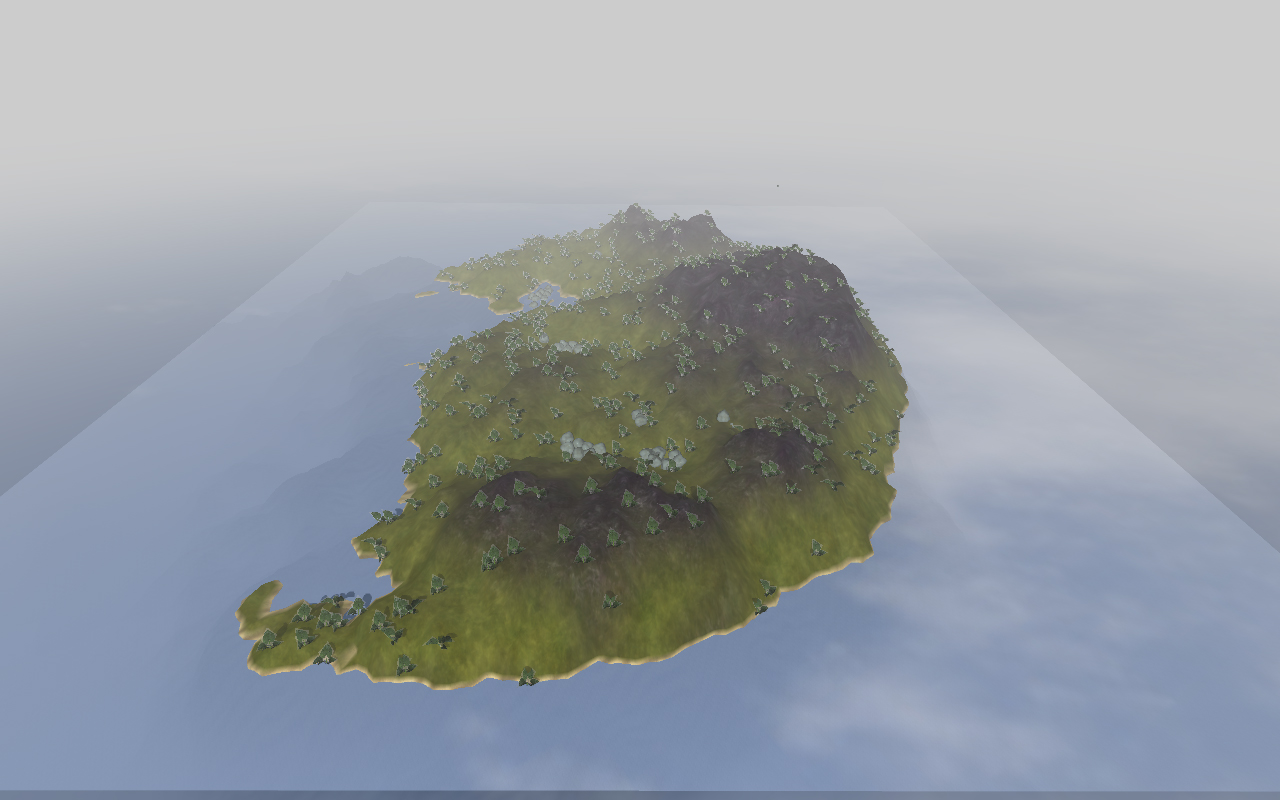
\includegraphics[width=0.9\linewidth]{images/SMOverViewLvl1.jpg}
  \caption{Shadow mapping level 1}
  \label{fig:SMOverViewLvl1}
\end{subfigure}%
\begin{subfigure}{.33\textwidth}
  \centering
  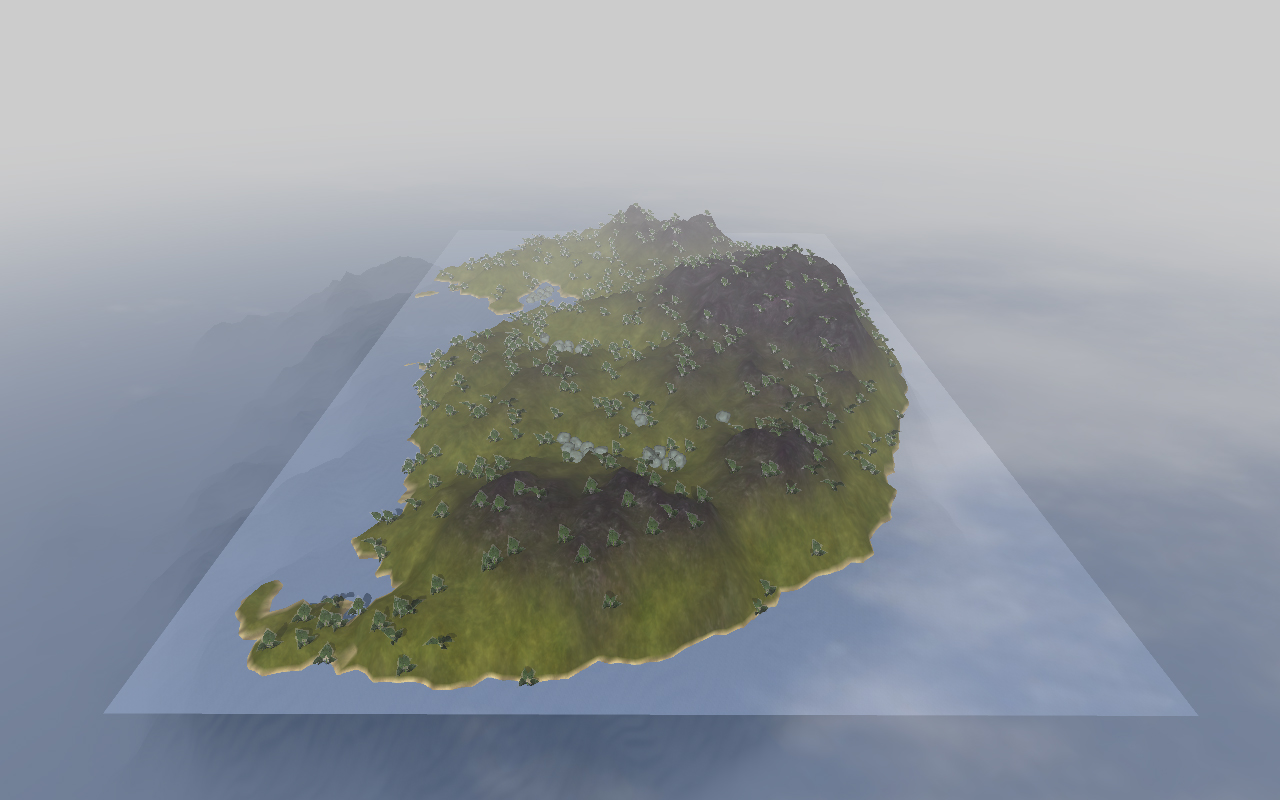
\includegraphics[width=0.9\linewidth]{images/SMOverViewLvl2.jpg}
  \caption{Shadow mapping level 2}
  \label{fig:SMOverViewLvl2}
\end{subfigure}
\begin{subfigure}{.33\textwidth}
  \centering
  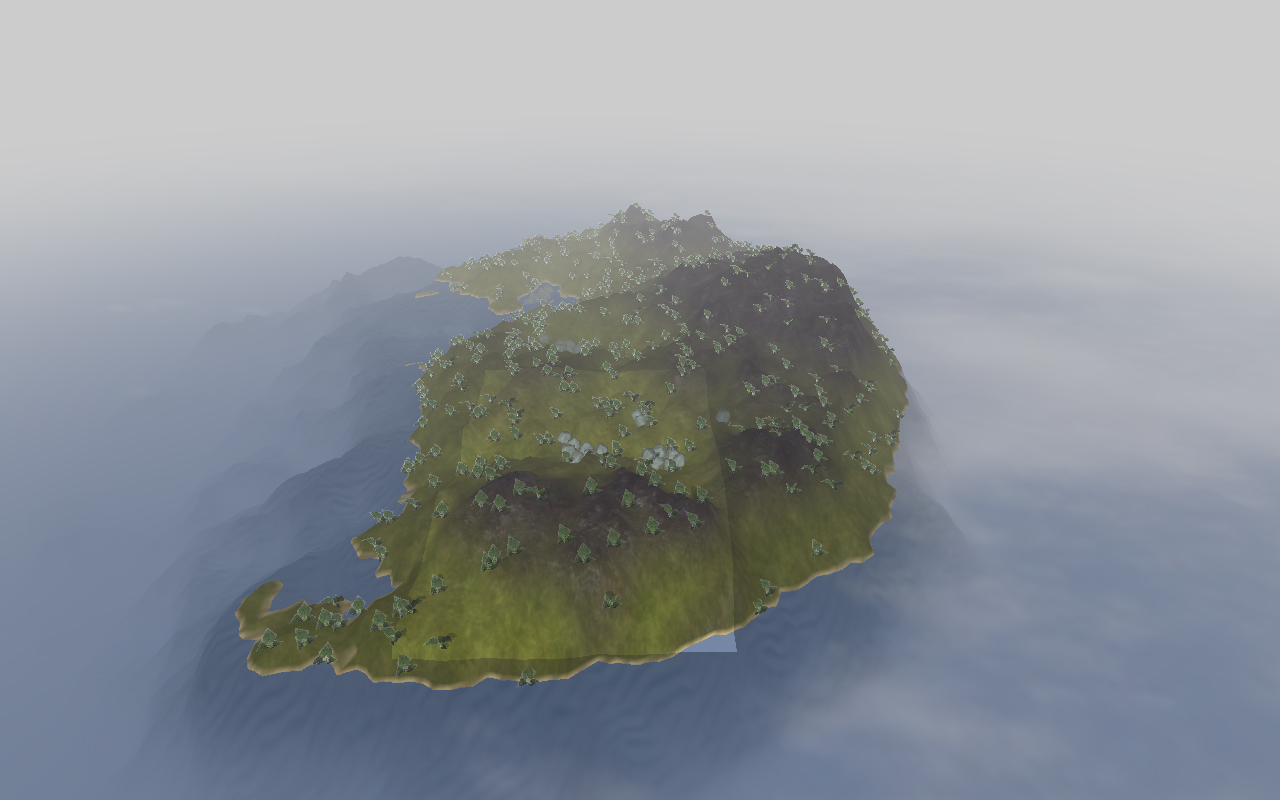
\includegraphics[width=0.9\linewidth]{images/SMOverViewLvl3.jpg}
  \caption{Shadow mapping level 3}
  \label{fig:SMOverViewLvl3}
\end{subfigure}
\caption[Noise comparison]{\textit{Overview of different shadow mapping levels}}
\label{fig:SMOverViewComparison}
\end{figure}

\begin{figure}[H]
\begin{subfigure}{.33\textwidth}
  \centering
  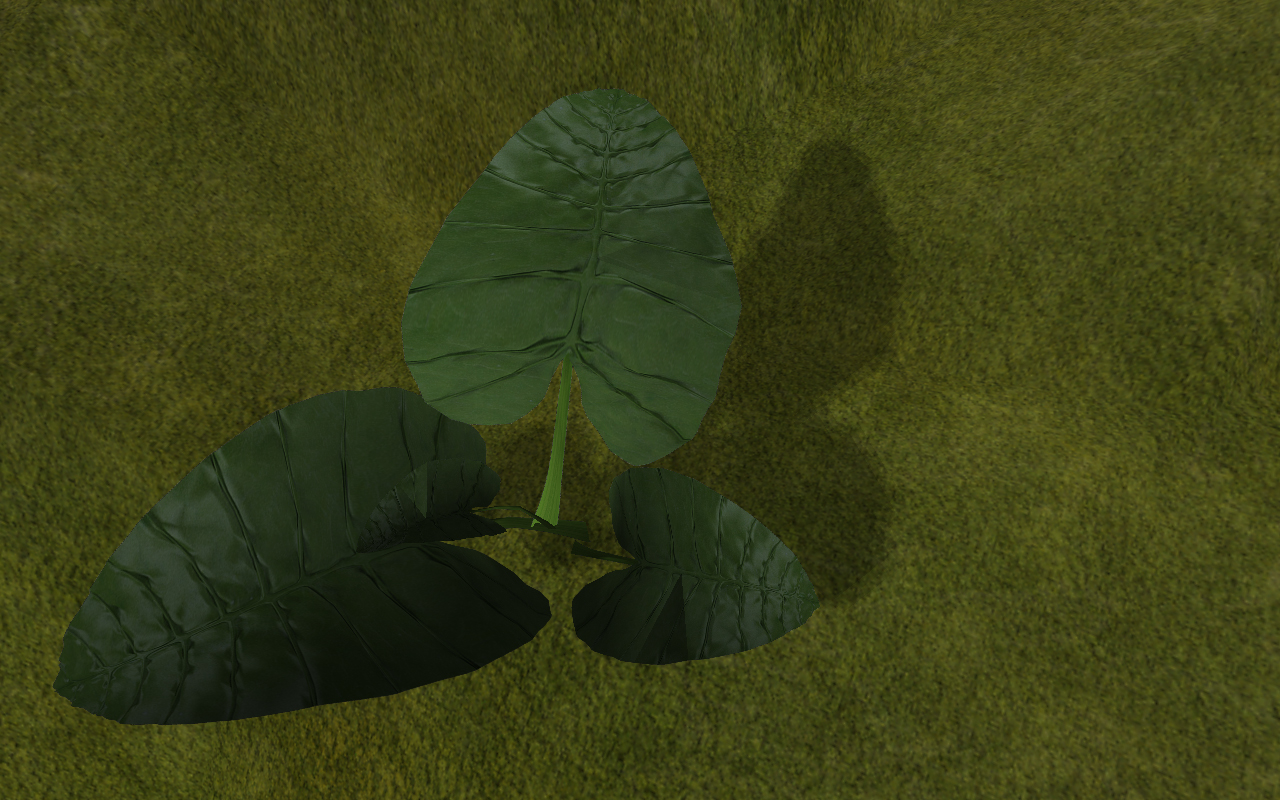
\includegraphics[width=0.9\linewidth]{images/SMCloseUpLvl1.jpg}
  \caption{Shadow mapping level 1}
  \label{fig:SMCloseUpLvl1}
\end{subfigure}%
\begin{subfigure}{.33\textwidth}
  \centering
  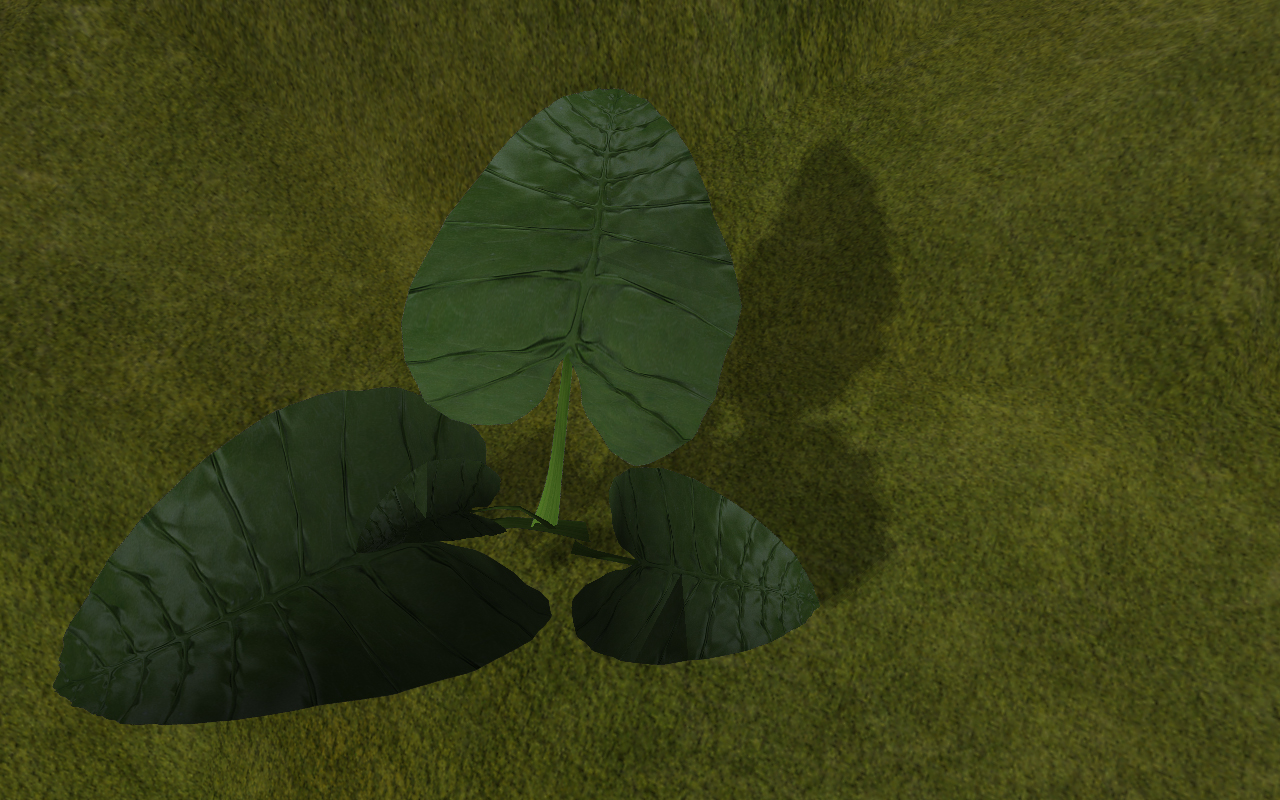
\includegraphics[width=0.9\linewidth]{images/SMCloseUpLvl2.jpg}
  \caption{Shadow mapping level 2}
  \label{fig:SMCloseUpLvl2}
\end{subfigure}
\begin{subfigure}{.33\textwidth}
  \centering
  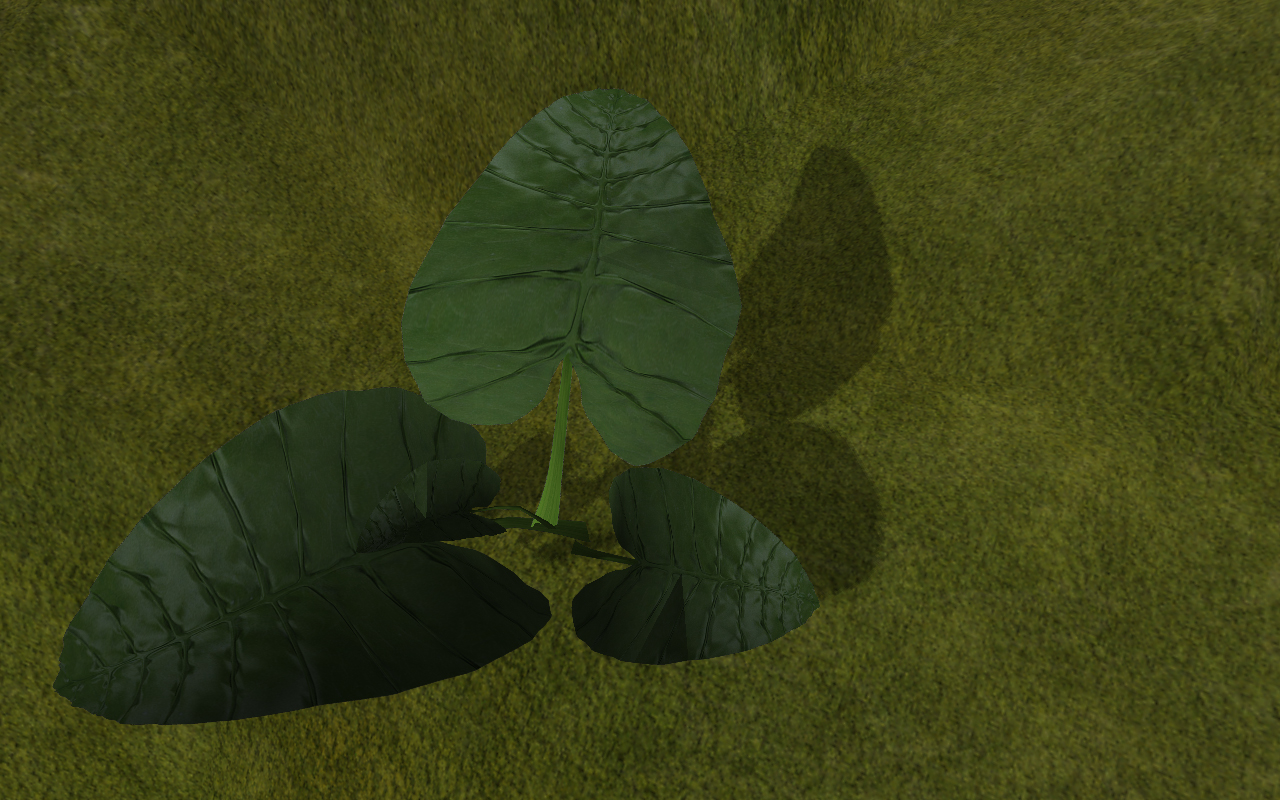
\includegraphics[width=0.9\linewidth]{images/SMCloseUpLvl3.jpg}
  \caption{Shadow mapping level 3}
  \label{fig:SMCloseUpLvl3}
\end{subfigure}
\caption[Noise comparison]{\textit{Close-up of different shadow mapping levels}}
\label{fig:SMCloseUpComparison}
\end{figure}

It would as conclusion be interesting to take a look at some modern examples, more precisely BattleField 3 (2011), Counter Strike: Global Offensive (2012), SimCity (2013) and League of Legends (2014). One can see that all of these are using shadow mapping in one way or another. The first three are using CSM and PCF combined to improve their shadows, but all are still suffering from ugly transitions between their cascade levels. SimCity holds a nice example of \textit{Perspective Aliasing} \cite{ImprovedShadowMapping}. League of Legends uses the simplest out-of-the-box version with no filtering or cascading at all. My point is: this is the way to go according to the cutting-edge game industry. One can also conclude that real-time shadowing is far from a finished topic. In all of the above mentioned games it is easy to find artifacts from optimizations. These are highlighted and amplified in figure \ref{fig:SMExComparison} below.

\begin{figure}[H]
\begin{subfigure}{.5\textwidth}
  \centering
  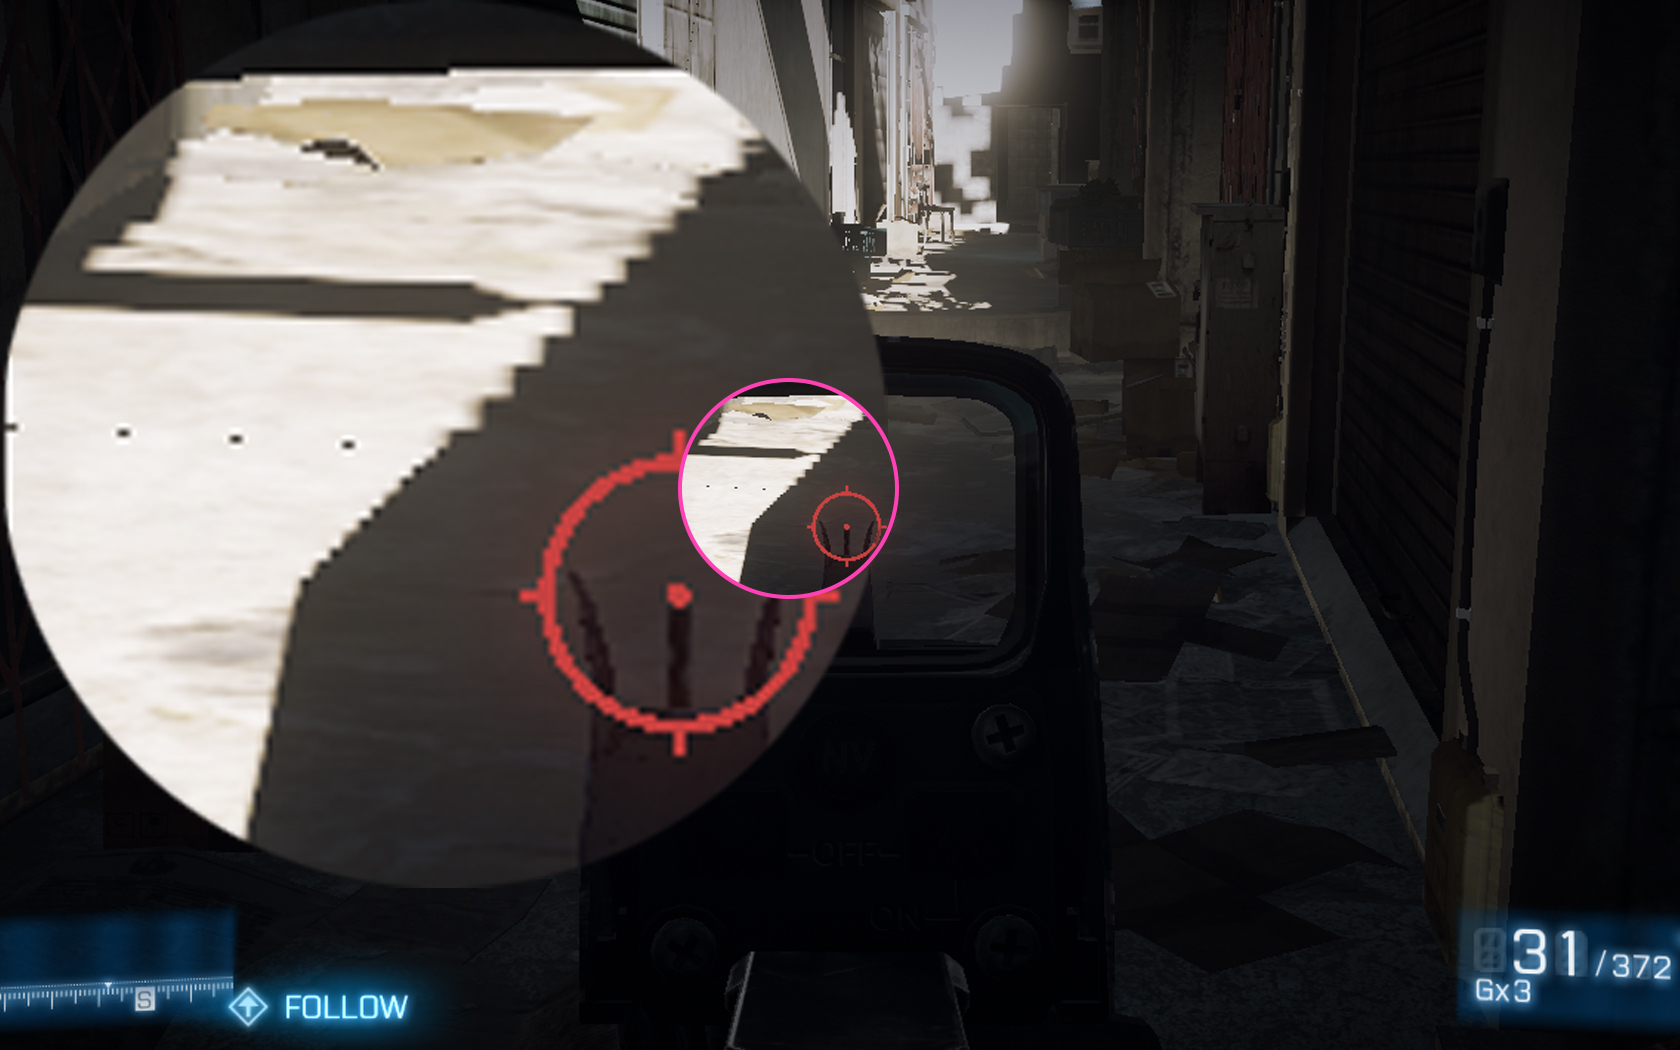
\includegraphics[width=0.9\linewidth]{images/SMExBF3.jpg}
  \caption{BattleField 3 (2011)}
  \label{fig:SMExBF3}
\end{subfigure}%
\begin{subfigure}{.5\textwidth}
  \centering
  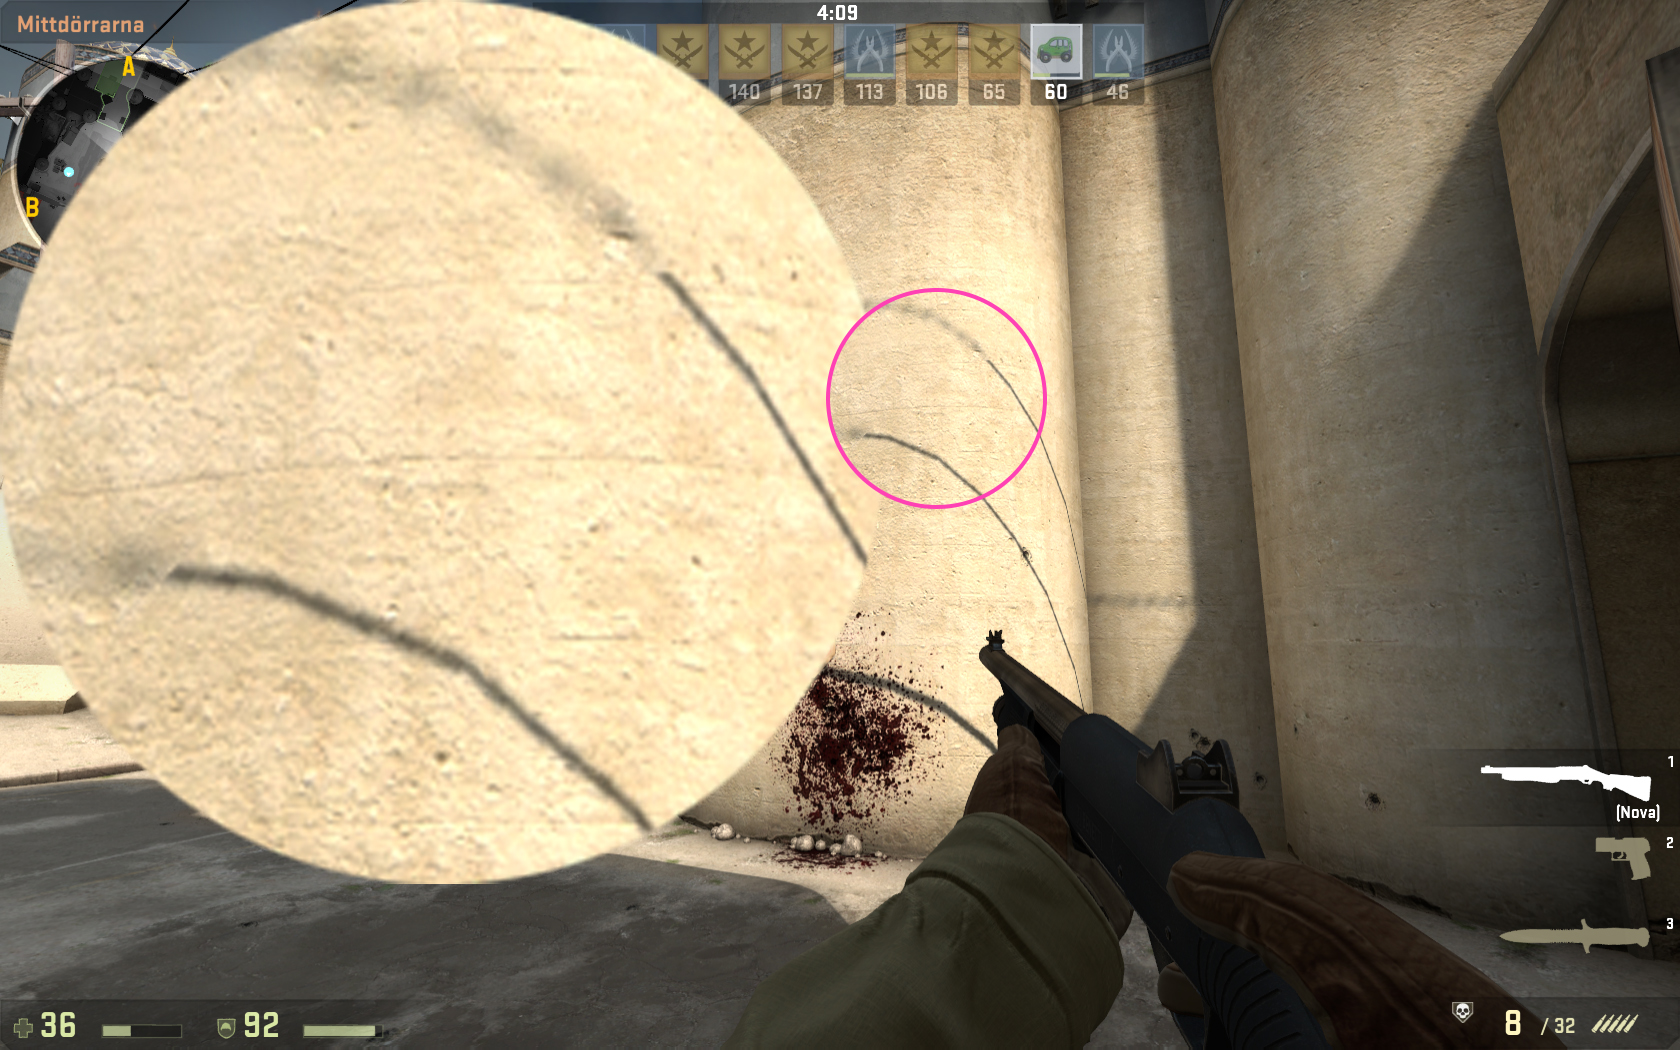
\includegraphics[width=0.9\linewidth]{images/SMExCSGO.jpg}
  \caption{Counter Strike: Global Offensive (2012)}
  \label{fig:SMExCSGO}
\end{subfigure}
\\
\begin{subfigure}{.5\textwidth}
  \centering
  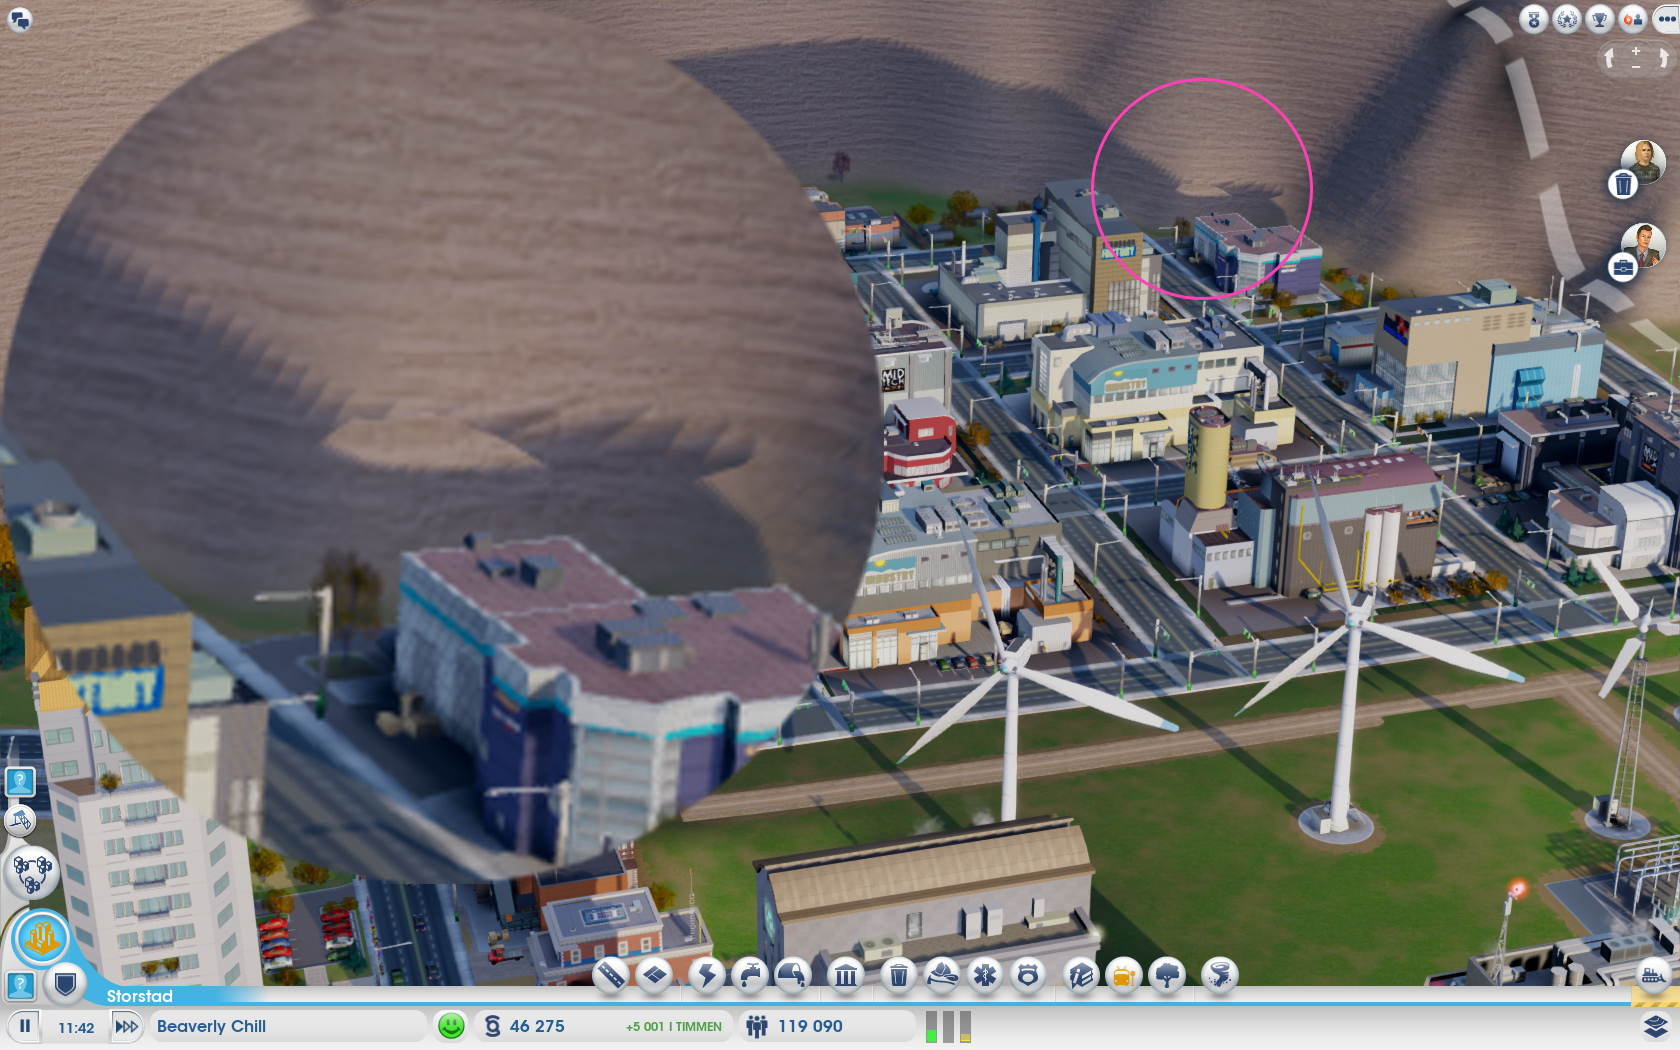
\includegraphics[width=0.9\linewidth]{images/SMExSimCity.jpg}
  \caption{SimCity (2013)}
  \label{fig:SMExSimCity}
\end{subfigure}%
\begin{subfigure}{.5\textwidth}
  \centering
  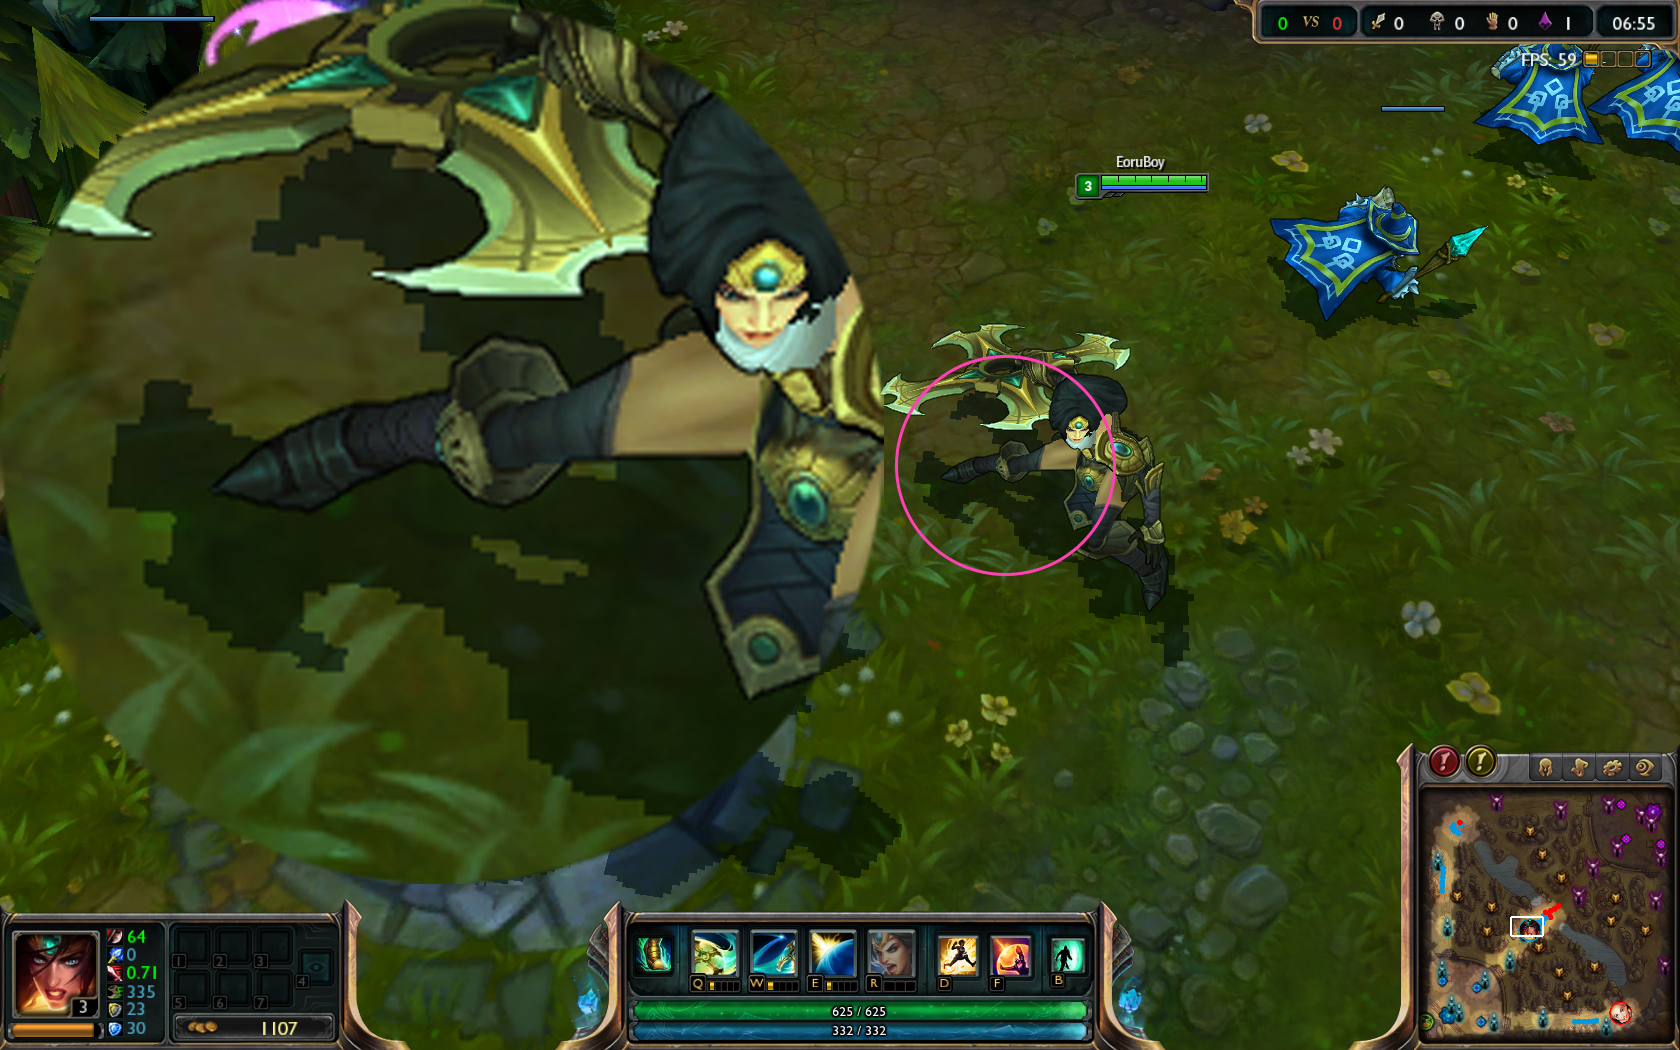
\includegraphics[width=0.9\linewidth]{images/SMExLoL.jpg}
  \caption{League of Legends (2014)}
  \label{fig:SMExLoL}
\end{subfigure}
\caption[Game industry standard shadow quality comparison]{\textit{Comparison of current game industry standard shadow quality}}
\label{fig:SMExComparison}
\end{figure}
\newpage
Our final in-game results can be seen in figure \ref{fig:InGameShadowResult}.
\begin{figure}[H]
\begin{subfigure}{.9\textwidth}
  \centering
  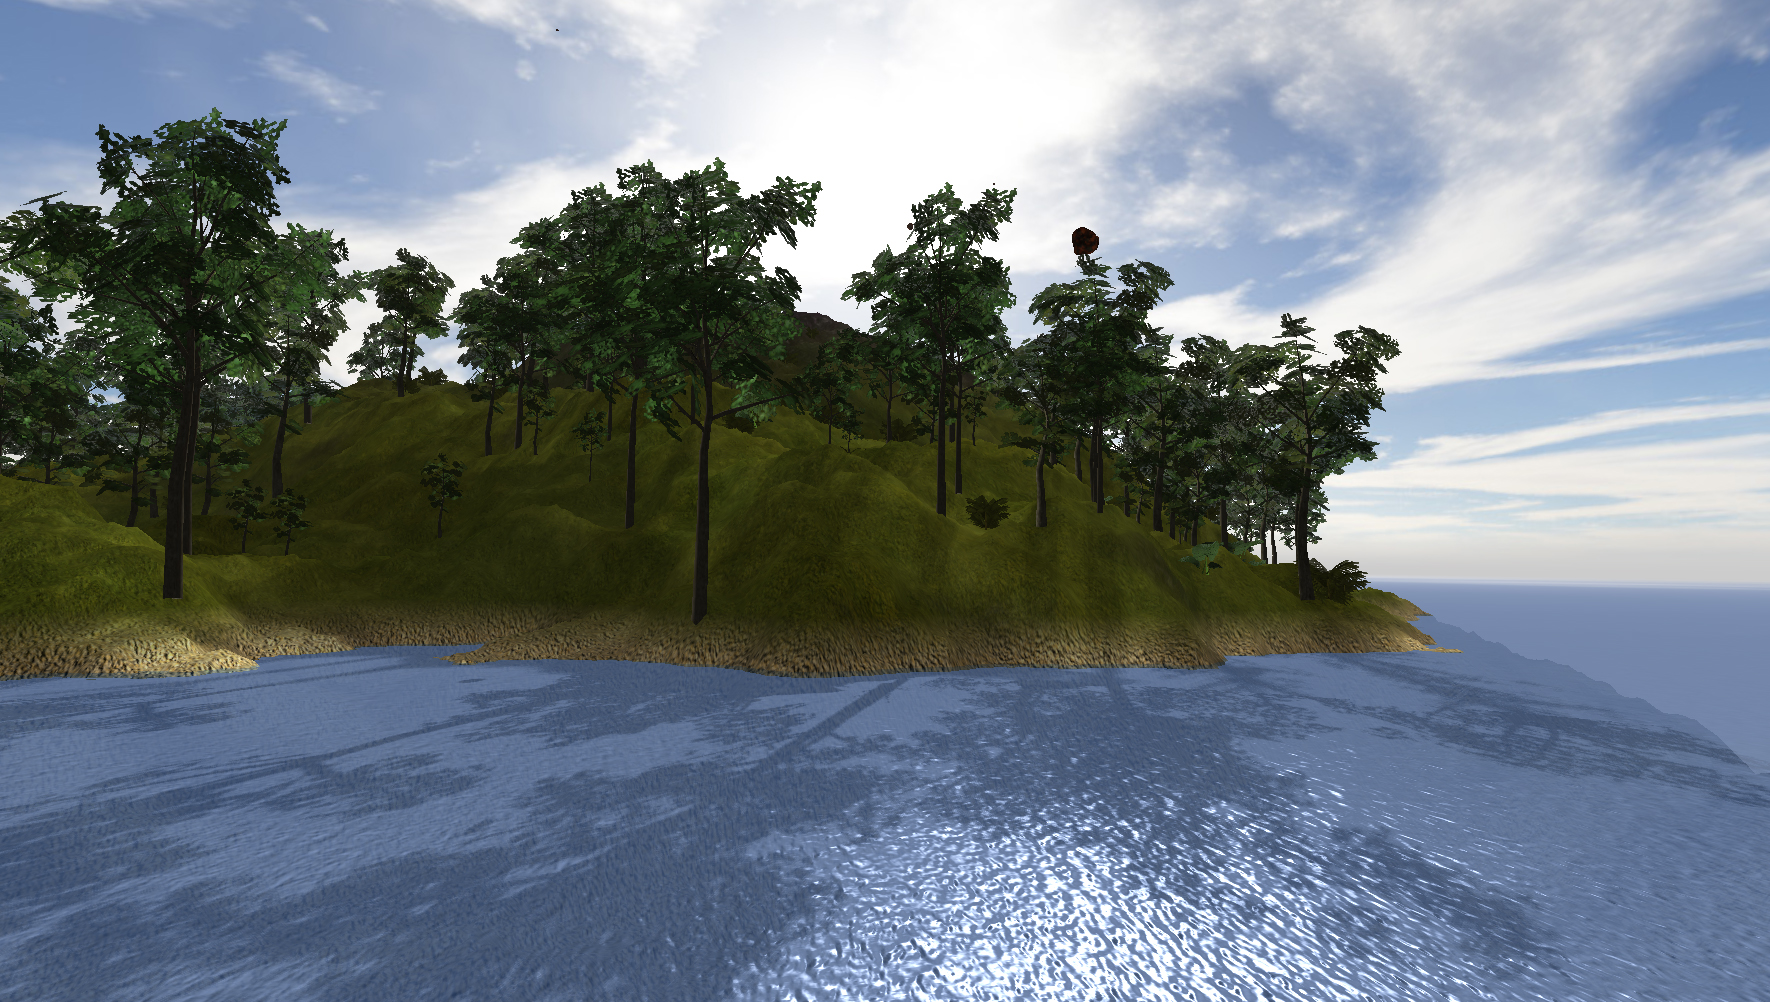
\includegraphics[width=0.9\linewidth]{images/shadows1.jpg}
  \caption{From the side, looking into the sun.}
  \label{fig:shadows1}
\end{subfigure}%
\\
\begin{subfigure}{.9\textwidth}
  \centering
  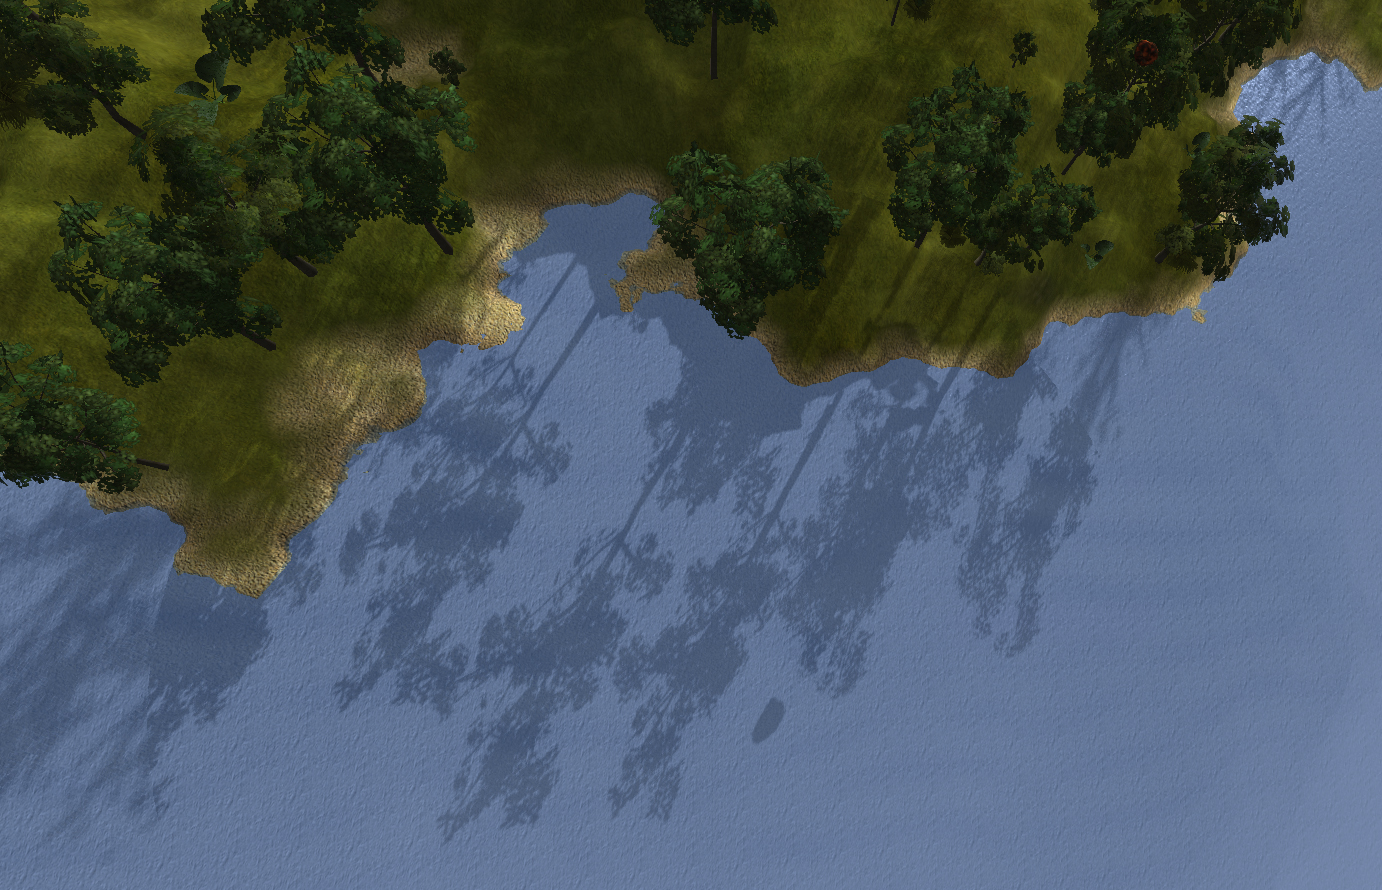
\includegraphics[width=0.9\linewidth]{images/shadows2.jpg}
  \caption{From the top.}
  \label{fig:shadows2}
\end{subfigure}
\caption{Two images of the same scene, showing our in-game shadow result. In (b) the cascade with the highest details do not cover the entire area, lower detail shadows can be seen to the left and to the top-right.}
\label{fig:InGameShadowResult}
\end{figure}

\newpage
\subsection{Distance fog}
The transition between different parts of the world can sometimes be very sharp in an unpleasant way. For instance, at the border between the sky and the ocean seen in figure \ref{fig:HorizonNoFog}. 

This can be remedied be adding some distance-fog to the ocean. If the color of the fog matches the color of the skybox at its horizon the transition will be seamless. Our skybox has been modify to fade into the color of the fog at its horizon, which can be seen in figure \ref{fig:SkyboxComparison} below. Notice that we have chosen to not let the skybox be affected by any fog. By doing so one can always see the sky when looking up, which is rather pleasant. 

\begin{figure}[H]
\begin{subfigure}{.5\textwidth}
  \centering
  \includegraphics[width=0.9\linewidth]{images/horizonNoFog.jpg}
  \caption{Horizon without fog}
  \label{fig:HorizonNoFog}
\end{subfigure}%
\begin{subfigure}{.5\textwidth}
  \centering
  \includegraphics[width=0.9\linewidth]{images/horizonFog.jpg}
  \caption{Horizon with fog}
  \label{fig:HorizonFog}
\end{subfigure}
\caption[Noise comparison]{\textit{Comparison of noise functions}}
\label{fig:HorizonFogComparison}
\end{figure}

\begin{figure}[H]
\begin{subfigure}{.5\textwidth}
  \centering
  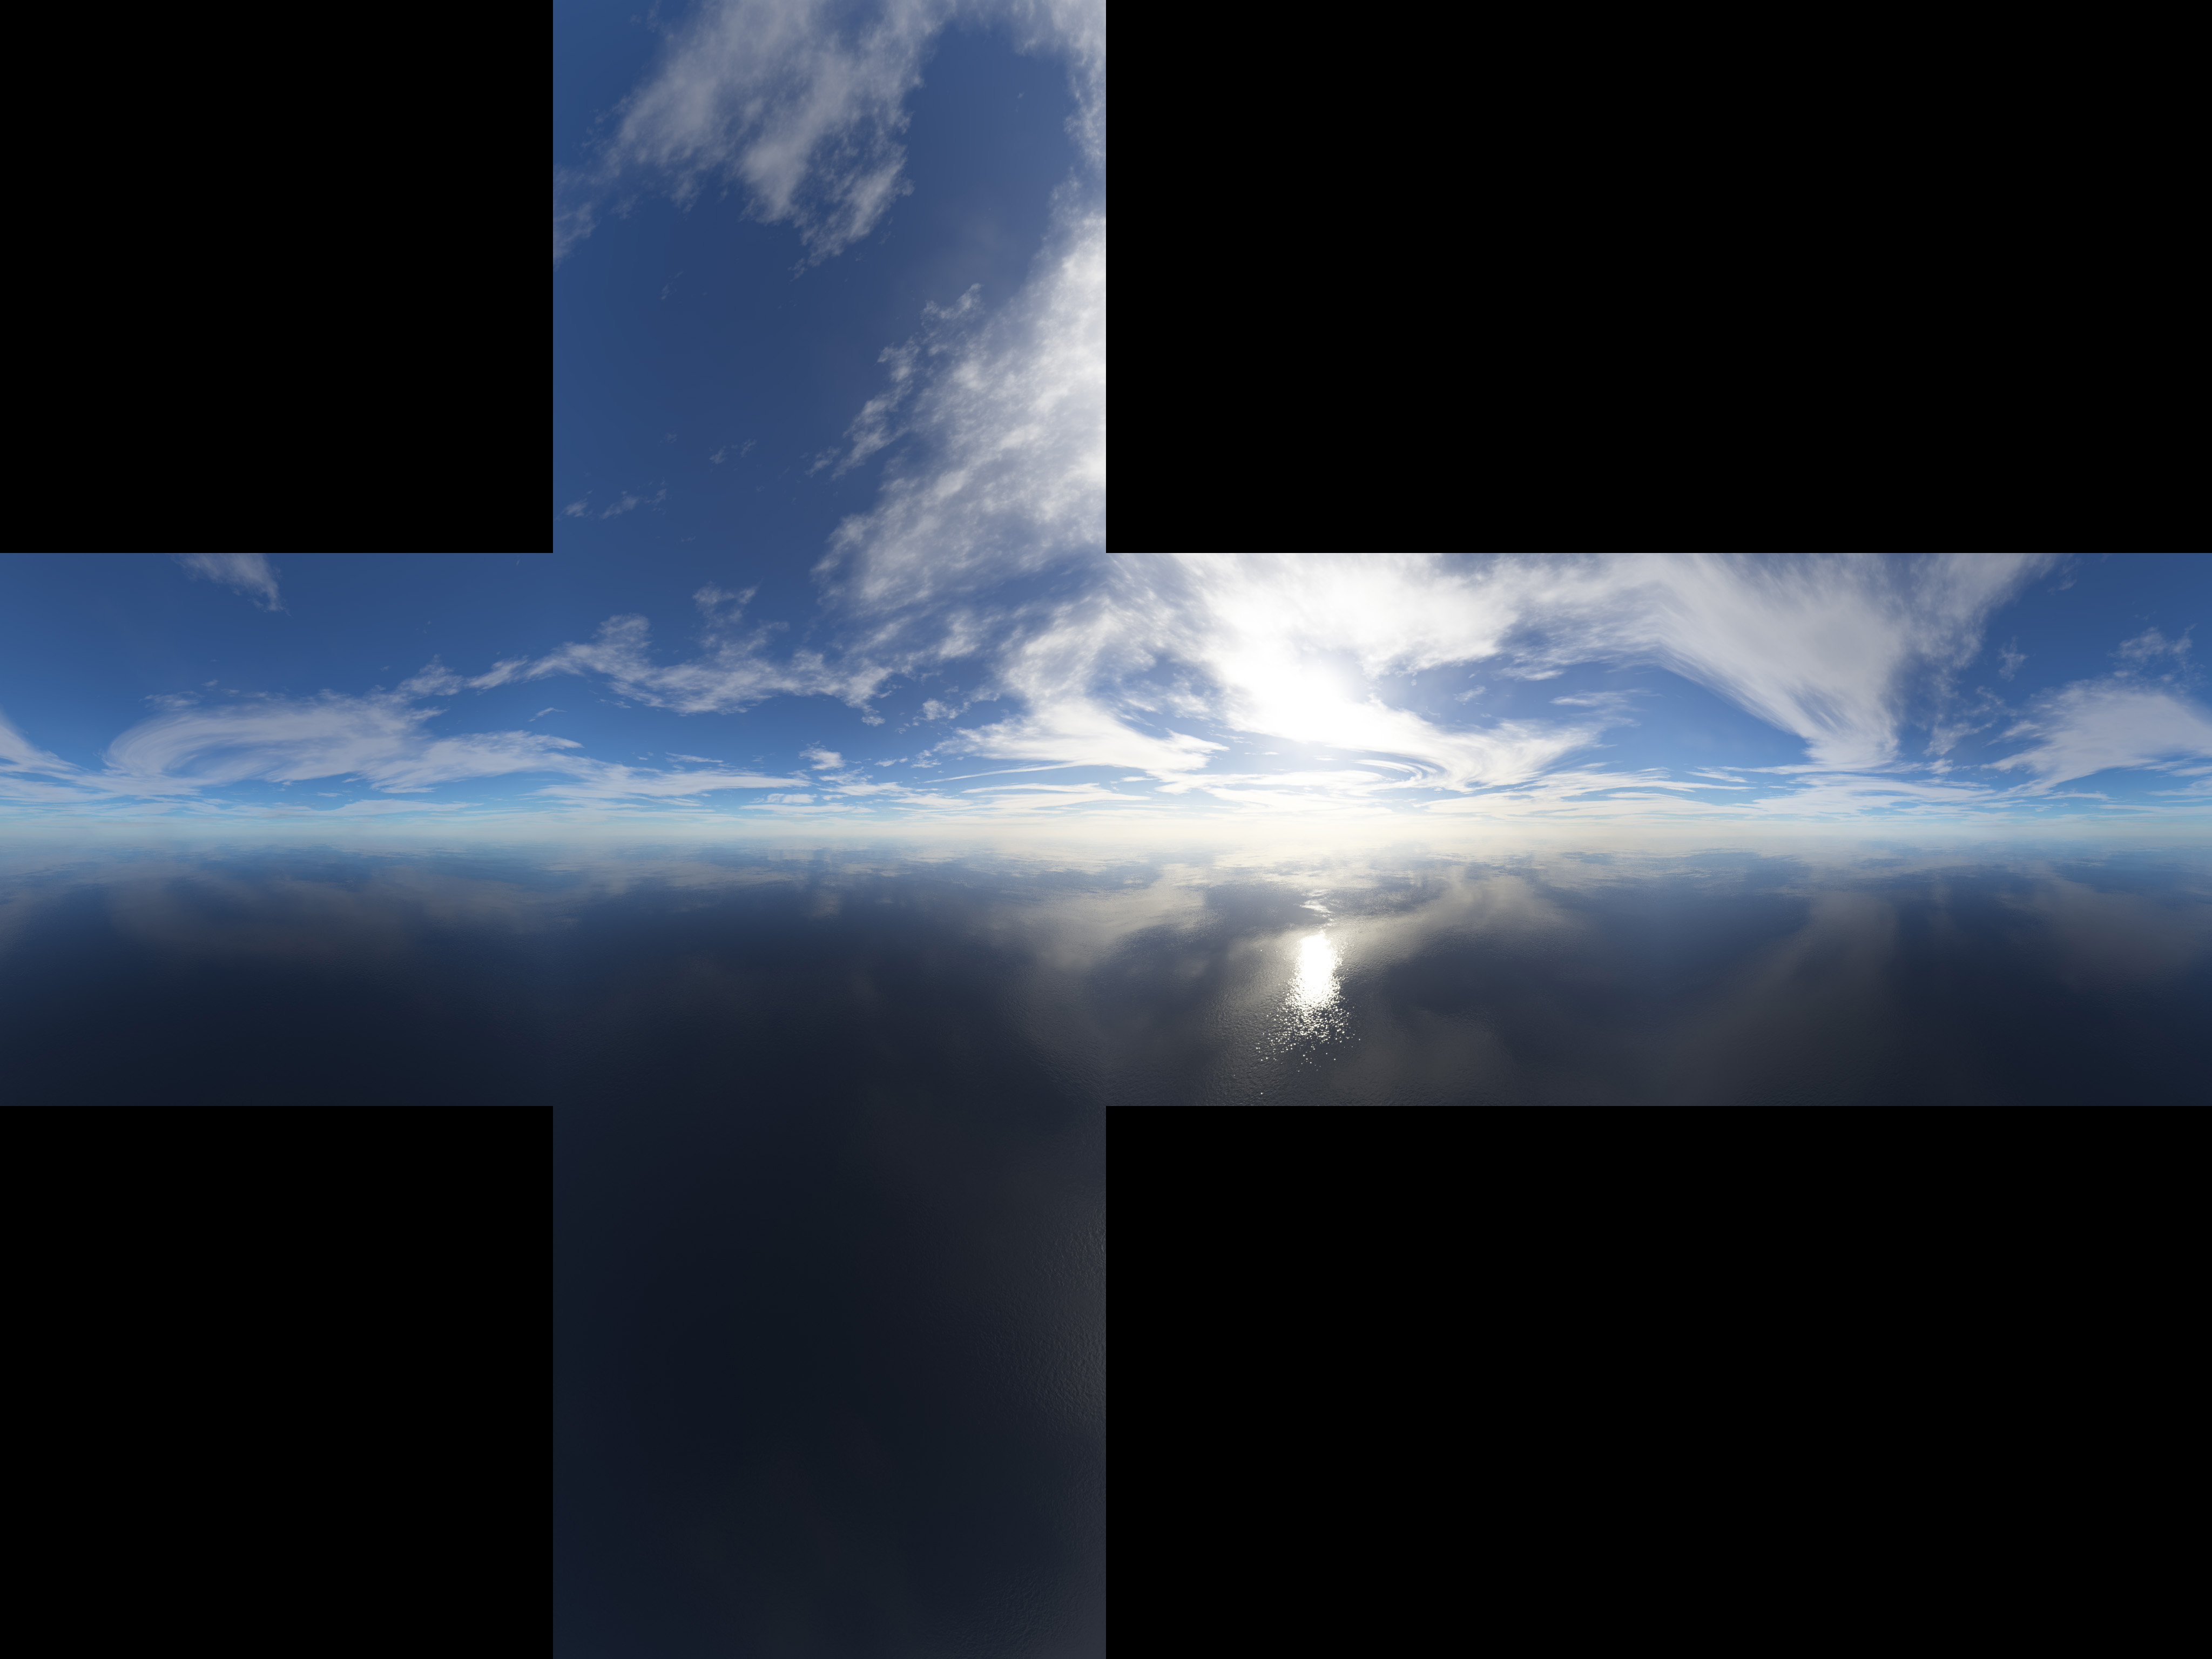
\includegraphics[width=0.9\linewidth]{images/skybox0.jpg}
  \caption{Original skybox}
  \label{fig:skybox0}
\end{subfigure}%
\begin{subfigure}{.5\textwidth}
  \centering
  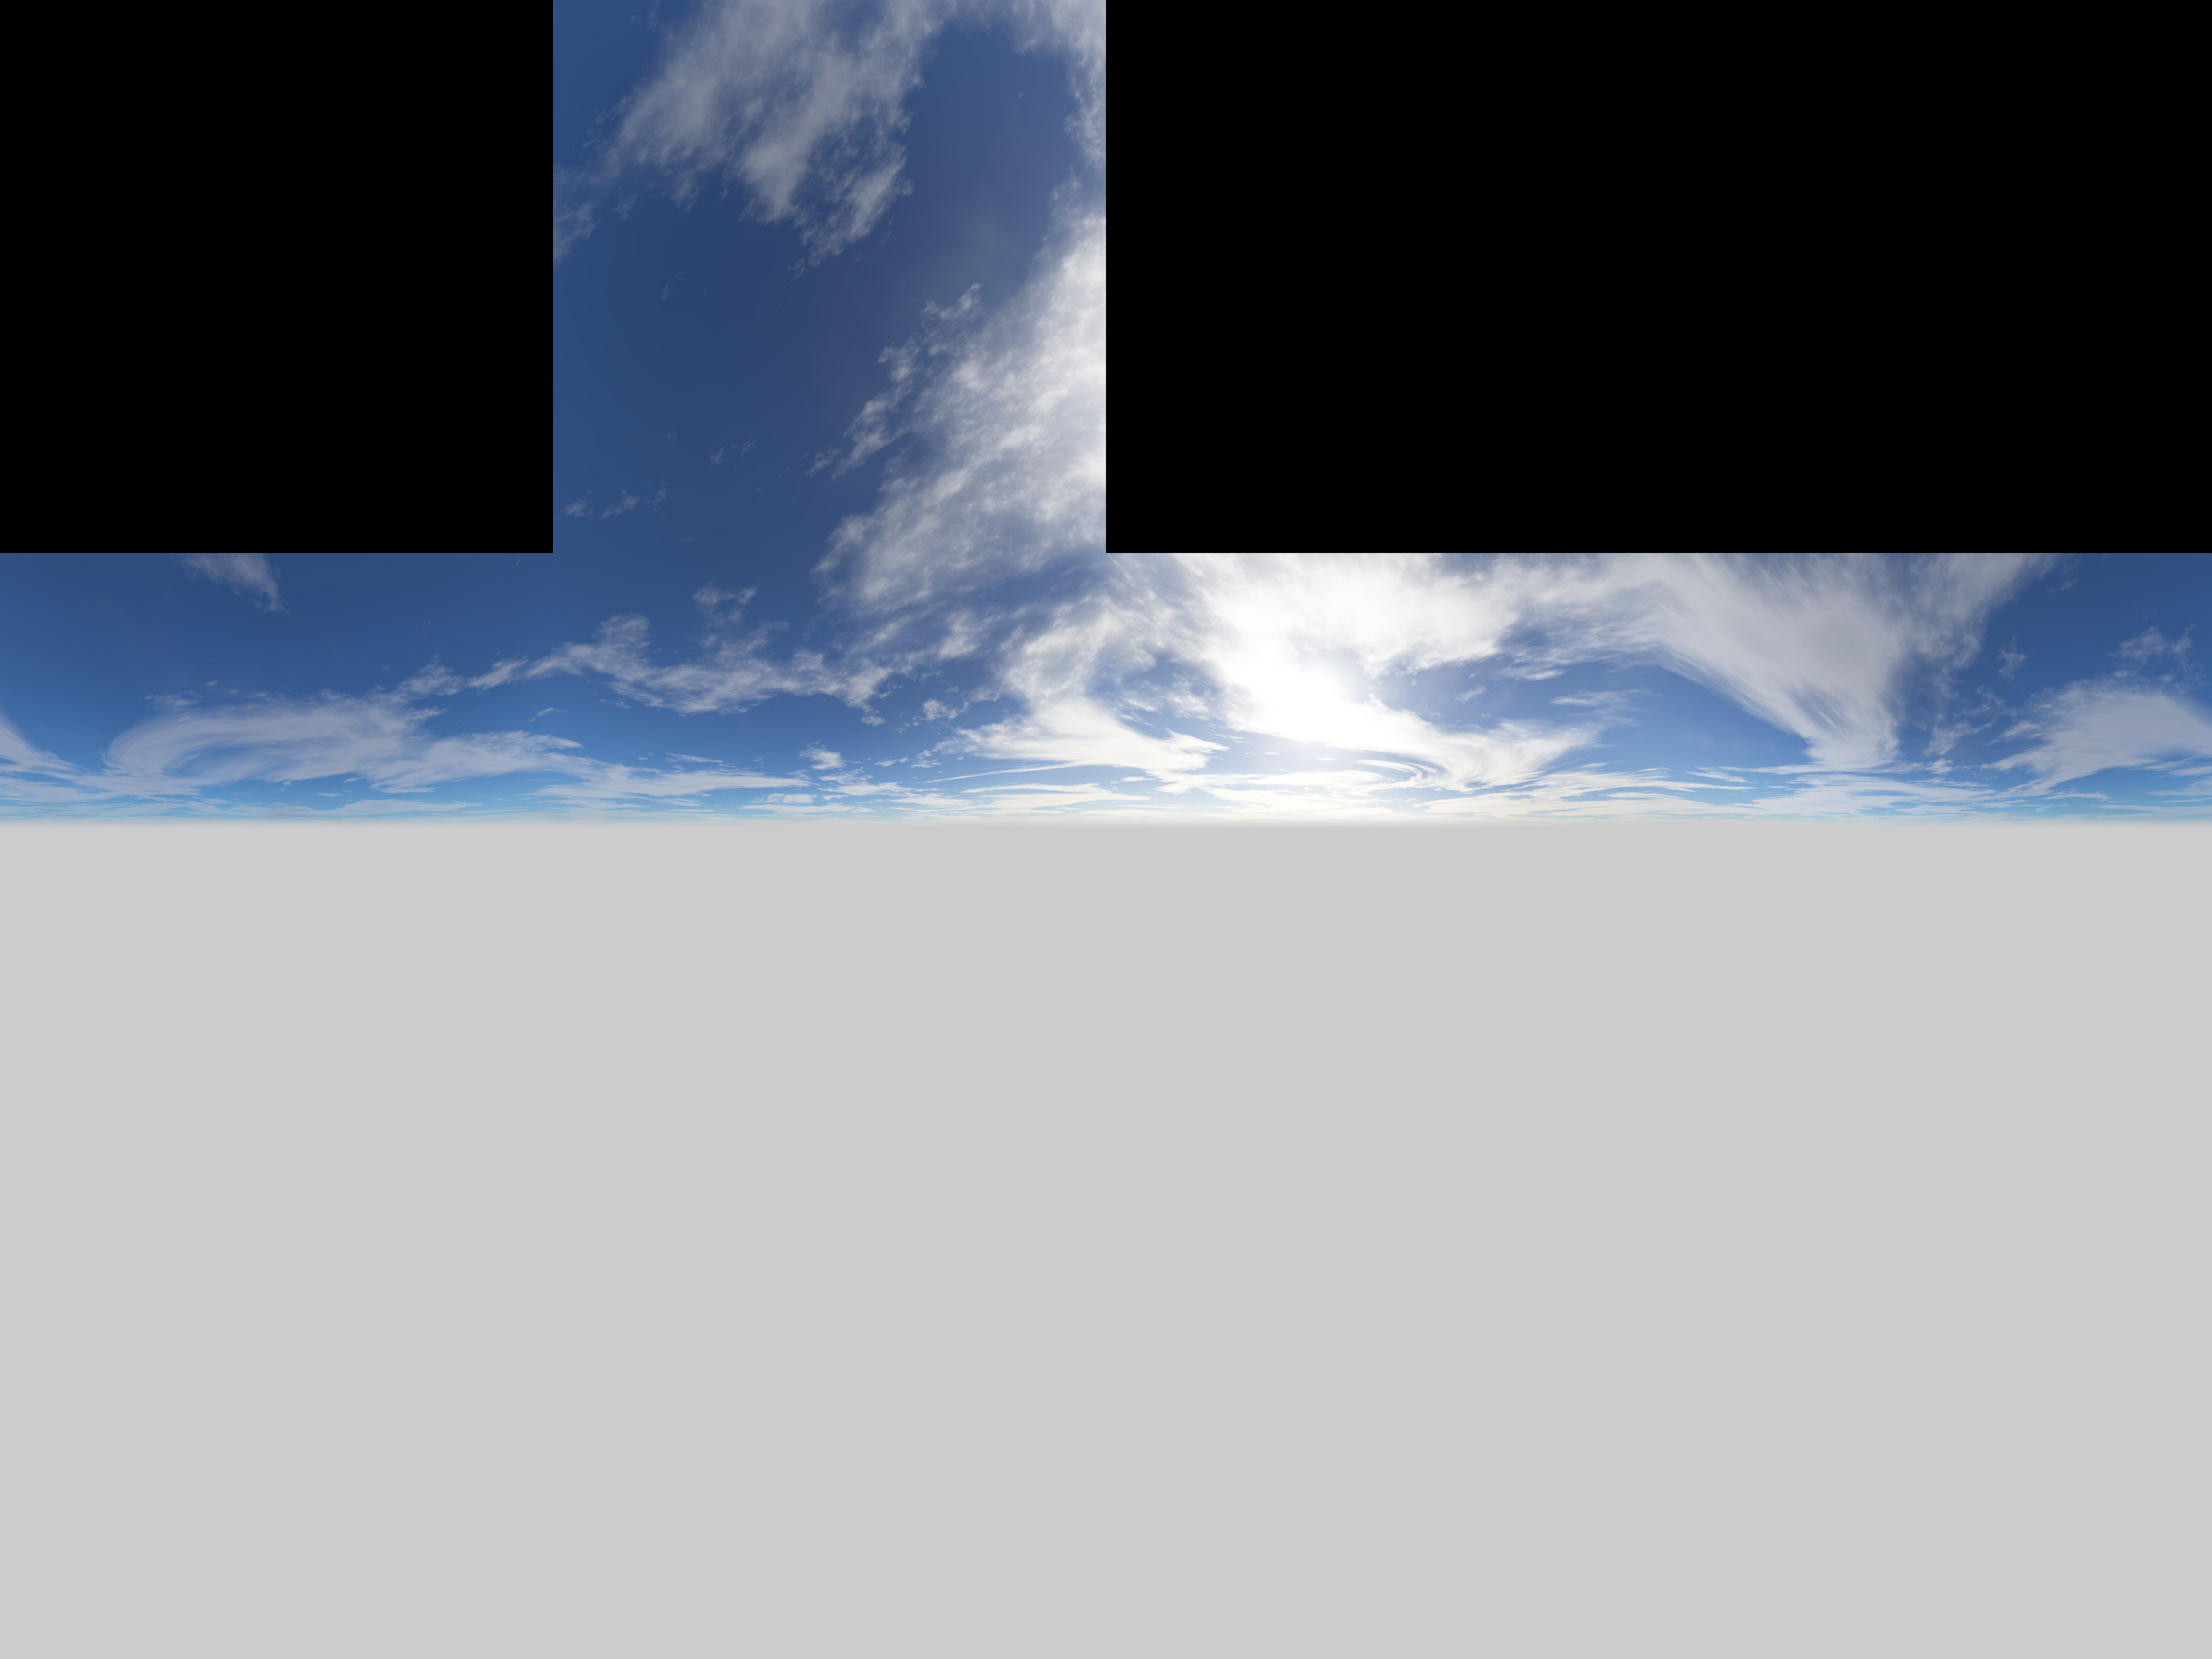
\includegraphics[width=0.9\linewidth]{images/skybox1.jpg}
  \caption{Skybox modified to fade into fog}
  \label{fig:skybox1}
\end{subfigure}
\caption[Noise comparison]{\textit{Comparison of skyboxes}}
\label{fig:SkyboxComparison}
\end{figure}

The distance-fog is also good for constraining the rendering size of the current scene. By adjusting the distance at which the fog appears one can adjust how much that is needed to be rendered of the scene. This enables an arbitrarily large world to be present without killing your computer since only the visible part of the world inside the fog-limit needs to be rendered. 

\newpage
\subsection{Normal Mapping}
Normal mapping is a technique for adding fine details to an object without adding more vertices, which saves a lot of geometry computations. A normal map is generally an image where the RGB-channels represent x,y and z coordinates for a normal vector. This texture is used in the fragment shader when computing the shading for the current fragment. Before calculating the shading the normal vector is rotated to match the object on which it is to be mapped. Notice that the normal vector is not translated since we want it to remain as an normalized direction and nothing more. A normal map is often used in combination with a texture, to give the texture an illusion of depth. An example of a normal map can be seen in figure \ref{fig:normalMapExample}.
\begin{figure}[H]
\begin{subfigure}{.5\textwidth}
  \centering
  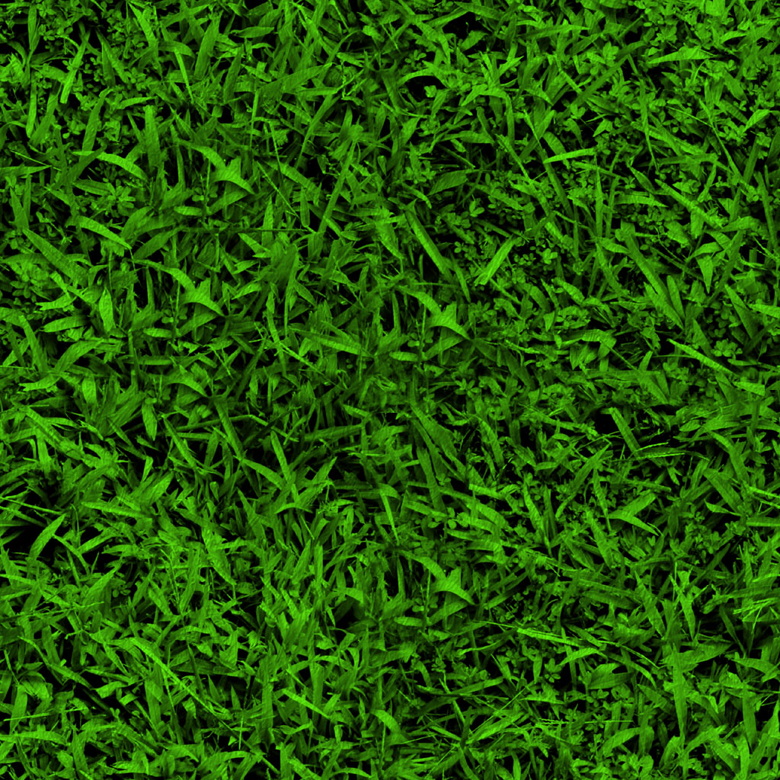
\includegraphics[width=0.9\linewidth]{images/grass1.jpg}
  \caption{Grass texture.}
  \label{fig:normalMapExampleGrassTexture}
\end{subfigure}%
\begin{subfigure}{.5\textwidth}
  \centering
  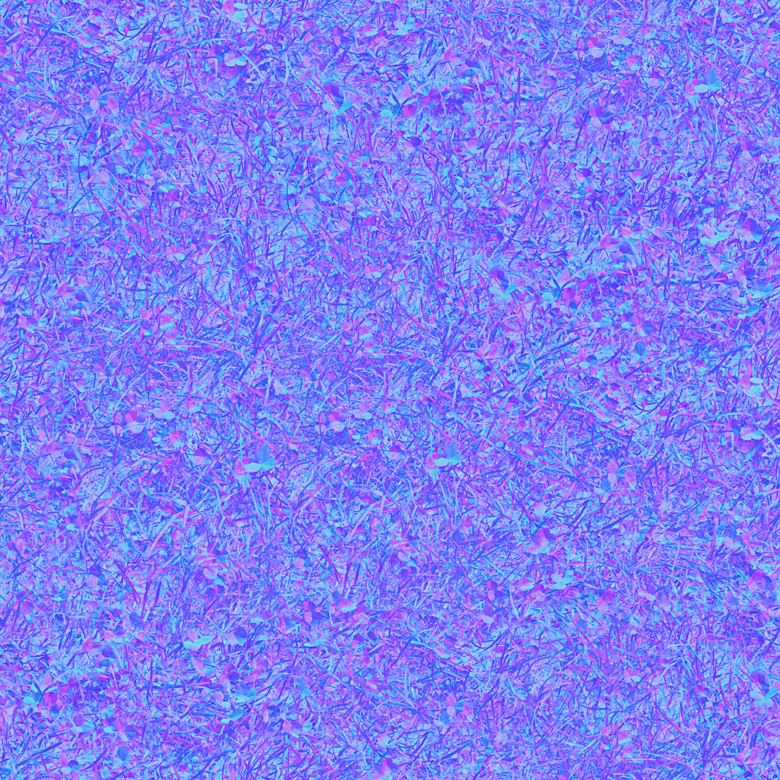
\includegraphics[width=0.9\linewidth]{images/grass1NormalMap.jpg}
  \caption{Grass normal map.}
  \label{fig:normalMapExampleGrassNormalmap}
\end{subfigure}
\caption[Normal Map example]{\textit{Example of a normal map.}}
\label{fig:normalMapExample}
\end{figure}